% begin module max-min-ex1
\begin{frame}
\begin{question}
Is it possible that a function attains its maximum/minimum value for infinitely many values of $x$?
\end{question}
\uncover<2->{
\begin{example}
The function $\cos x$ attains its maximum value (=$1$) infinitely many times, since $\cos (2n \pi) = 1$ for any integer $n$.

Likewise, it attains its minimum value of $-1$ infinitely many times, because $\cos \left((2n+1)\pi\right) = -1$ for all integers $n$.

\psset{xunit=0.7cm, yunit=0.7cm}
\begin{pspicture}(-5.5,-1.7)(11.4,1.9)
\tiny
\psframe*[linecolor=white](-5.5,-1.7)(11.4,1.9)
\psaxes[ticks=x, tickstyle=top, Dx=3.1415, labels=none]{<->}(0,0)(-5.5,-1.7)(11.2,1.7)
%Function formula: \cos{}(x) 
\rput(3,1){$y=\cos{}(x)$} 
\psplot[linecolor=red, plotpoints=1000]{-5}{11}{x 57.29578 mul cos }
\rput[t](-3.1415, -0.15){$-\pi$}
\rput[t](-1.570796327, -0.15){$-\frac{\pi}{2}$}
\rput[t](1.570796327, -0.15){$\frac{\pi}{2}$}
\rput[t](3.1415, -0.15){$\pi$}
\rput[t](4.71238898, -0.15){$\frac{3\pi}2$}
\rput[t](6.283185307, -0.15){$2\pi$}
\rput[t](7.853981634, -0.15){$\frac{5\pi}{2}$}
\rput[t](9.424777961, -0.15){$3\pi$}
\end{pspicture} 
%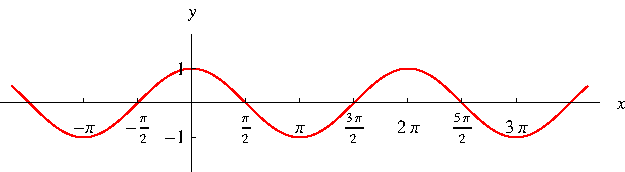
\includegraphics[width=12cm]{maxima-minima/pictures/app-d-cos.pdf}%
\end{example}
}
\end{frame}
% end module max-min-ex1